\documentclass[main.tex]{subfiles}
\begin{document}
\subsection{The waving of hands}
This section will informally give a basic idea for all concepts used throughout the text
with the sole purpose to give some intuition about the project end-to-end.

Our goal is to have our user write a query like this:
\begin{center}
    \code{pharmacies near parking spaces in Berlin}
\end{center}
And get such circles on a map as those shown in \cref{fig:circles}.

\cfigure{
    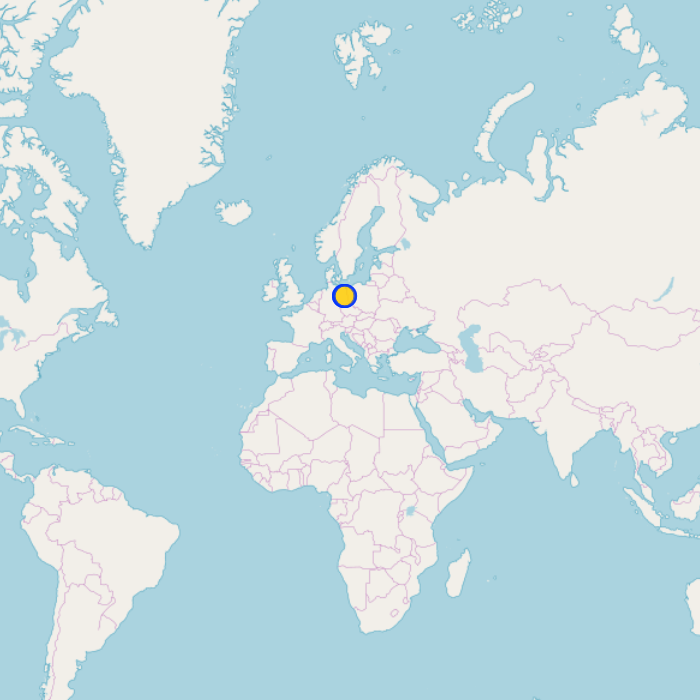
\includegraphics[width=0.32\textwidth]{map/world.png}
    \hfill
    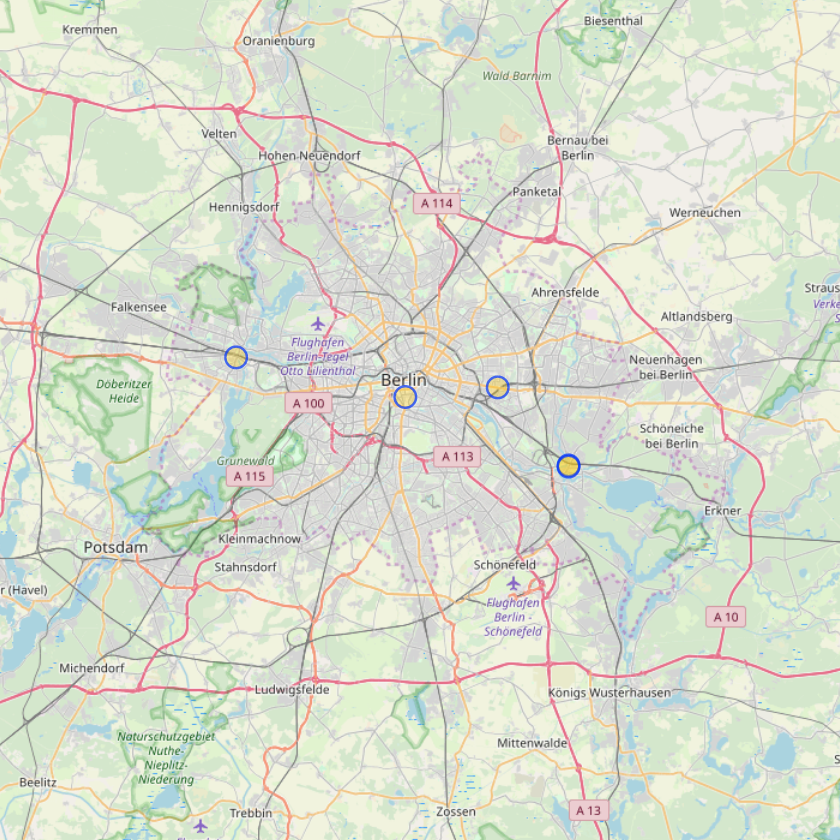
\includegraphics[width=0.32\textwidth]{map/berlin.png}
    \hfill
    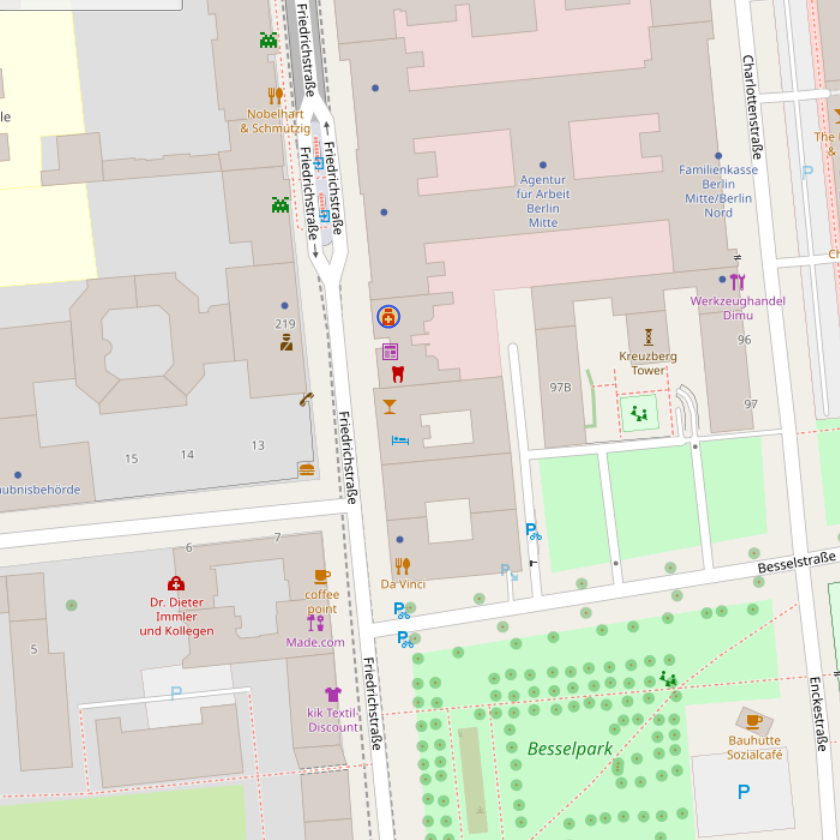
\includegraphics[width=0.32\textwidth]{map/pharmacy.png}
    \caption{Wanted result for query ``pharmacies near parking spaces in Berlin''}
    \label{fig:circles}
}

To do this, we will first construct a Combinatory Categorial Grammar which parses
such queries. The central idea of CCG is that each word (or terminal) is assigned
a set of
\emph{categories}, which work the same way as types work in programming
languages\footnote{Especially curried programming languages like Haskell}.
Semantically, each word returns something and may take other things as arguments.

Here, our basic type will be called $GSet$ and will mean "a set of geographic
objects". Each basic type is also a category.

So, we can immediately assign the category of \code{pharmacies} and of
\code{Berlin} to be $GSet$ - they will have the semantics of ``the set of all
pharmacies'' and ``the singleton of the city of Berlin'' respectively:
\gramshort{
    \gramrow{pharmacies}{ GSet }{}
    \gramrow{Berlin}{ GSet }{}
}

Now, we want \code{parking spaces} to have a $GSet$ category and the semantics
of ``the set of all parking spaces''. One way to do this is to assign a special
category $Spaces$ to the word \code{spaces}, and make \code{parking} take
$Spaces$ as an argument on the right and returns $GSet$. We will denote this
``argument on the right'' construction by a forward slash:
\gramshort{
    \gramrow{parking}{ GSet \rc Spaces }{}
    \gramrow{spaces}{Spaces}{}
}
Coincidentally, arguments on the left will be denoted by a backward slash.

Now, we need to assign a category to the word \code{in}. We want to parse
the construction ``something in something'', thus we want to take one $GSet$
on the left and one $GSet$ on the right, and return another $GSet$:
\gramshort{
    \gramrow{in}{ (GSet \lc GSet) \rc GSet }{}
}
This means that \code{in} will take a $GSet$ on the right and produce something
which takes another $GSet$ on the left and returns the final $GSet$.
In our case, \code{in Berlin} takes something of type $GSet$ on the left and
returns a $GSet$.
An alternative category that would also work is the following:
\gramshort{
    \gramrow{in}{ (GSet \rc GSet) \lc GSet }{}
}
In this case, \code{in Berlin} makes no sense, but \code{parking spaces in}
will return something that will gladly take \code{Berlin} on the right and
produce a $GSet$.

The syntax of ``near'' is similar to the syntax of ``in'', so we will assign
the same category. Finally, we get this simple grammar:
\gramshort{
    \gramrow{pharmacies}{ GSet }{}
    \gramrow{Berlin}{ GSet }{}
    \gramrow{parking}{ GSet \rc Spaces }{}
    \gramrow{spaces}{Spaces}{}
    \gramrow{in}{ (GSet \lc GSet) \rc GSet }{}
    \gramrow{near}{ (GSet \lc GSet) \rc GSet }{}
}
Which will parse our query. The most convenient way to illustrate such parses
is by means of a \emph{derivation tree}:
\centree{.{$GSet$}
    [ .{$GSet$}
        [ .{$GSet$} [ .{$pharmacies$} ] ]
        [ .{$GSet \lc GSet$}
            [ .{$(GSet \lc GSet) \rc GSet$} [ .{$near$} ] ]
            [ .{$GSet$}
                [ .{$GSet \rc Spaces$} [ .{$parking$} ] ]
                [ .{$Spaces$} [ .{$spaces$} ] ]
            ]
        ]
    ]
    [ .{$GSet \lc GSet$}
        [ .{$(GSet \lc GSet) \rc GSet$} [ .{$in$} ] ]
        [ .{$GSet$} [ .{$Berlin$} ] ]
    ]
}

\fixme{write some text}
\end{document}
